\section{Josep Maria Proposal}

\subsection{Requirements}

\paragraph{} First of all, we must take into account the requirements of our constellation. Those requirements are the following:
\pagebreak
\begin{table}[htb]
\centering
\begin{tabular}{c p{14cm}}
\toprule
\textbf{Feature} & \textbf{Description}                                                                                                                                                          \\ \midrule
1                & \begin{tabular}[c]{@{}l@{}}Provide communication relay between two LEO nanosatellites with a latency \\ \textbf{lower than 1 minute}.\end{tabular}\vspace{0.3cm}                                                 \\
2                & \begin{tabular}[c]{@{}l@{}}Provide communication relay between a LEO nanosatellite and the ground \\ with a latency \textbf{lower than 5 minutes.}.\end{tabular}\vspace{0.3cm}                                                                                        \\
3                & \begin{tabular}[c]{@{}l@{}}Back-up system prepared to handle \textbf{up to two major failures} in the system.\\ A major failure can be defined as the loss of a client’s satellite coverage because\\ of a failure in the network.\end{tabular}\vspace{0.3cm}                                                 \\
4                & \begin{tabular}[c]{@{}l@{}}Switch time after major failure happens, shall be\textbf{ below 6 hours}.\end{tabular}\vspace{0.3cm}                                                                                                     \\
5                & \begin{tabular}[c]{@{}l@{}}Each Satellite Node volume should be equal or \textbf{lower than a 3U Cubesat.}\end{tabular}\vspace{0.3cm}                                                                                                     \\
6                & \begin{tabular}[c]{@{}l@{}}Each Node should be able to handle \textbf{at least 25 Mbit/s} of data rate.\end{tabular}\vspace{0.3cm}                                                                                                     \\ \bottomrule
\end{tabular}
\caption{Project Requirements}
\end{table}

\paragraph{}The most restricting requirements are:

\begin{itemize}
\item Back-up system prepared to handle \textbf{up to two major failures} in the system.
\item Switch time after major failure happens, shall be\textbf{ below 6 hours}.
\end{itemize}

\paragraph{}This requirements limit the type of network architecture that can be implemented. A ring network will fail completely if two major failures isolate one segment from the rest of the ring. A star network will fail if the hub has a major failure. It has to be taken into account that 6 hours is not enough time to replace a satellite node. A full mesh network will simply not work because not all satellites are visible due to the Earth being in the middle of the constellation. This only leaves us with different kinds of hybrid networks. The proposal in this section is the implementation of a mesh-ring hybrid network.


\subsection{Network}

\paragraph{}For this proposal to be effective, the satellite constellation has to be done in a series of polar, or near polar, orbits where all planes move in the same direction. This will create two hemispheres where in one the satellites move from south to north, and in the other one they move from north to south. If there were two adjacent planes moving in opposite directions, the relative velocity of the satellites will be very high, and its relative position will also vary significantly, almost covering 180º. Aside from Doppler effects, this configuration will need a tracking system for two antennas or invest a lot of power in a antenna with very wide range, and since our satellites are cubesats of 3 units at maximum, it is preferable to not have this kind of systems.

\paragraph{}With this configuration, the general idea is to design a network where each satellite node has a link with four neighbouring ones. Two of this links will be with the next and previous satellite of the same orbital plane. The other two will be with be with a satellite in the two adjacent planes, with the exception of the orbital planes which neighbours will move in the other direction (one plane moving north-to-south, and the adjacent moving south-to-north). This links between satellites can be bi-directional.

\begin{figure}[H]
\centering
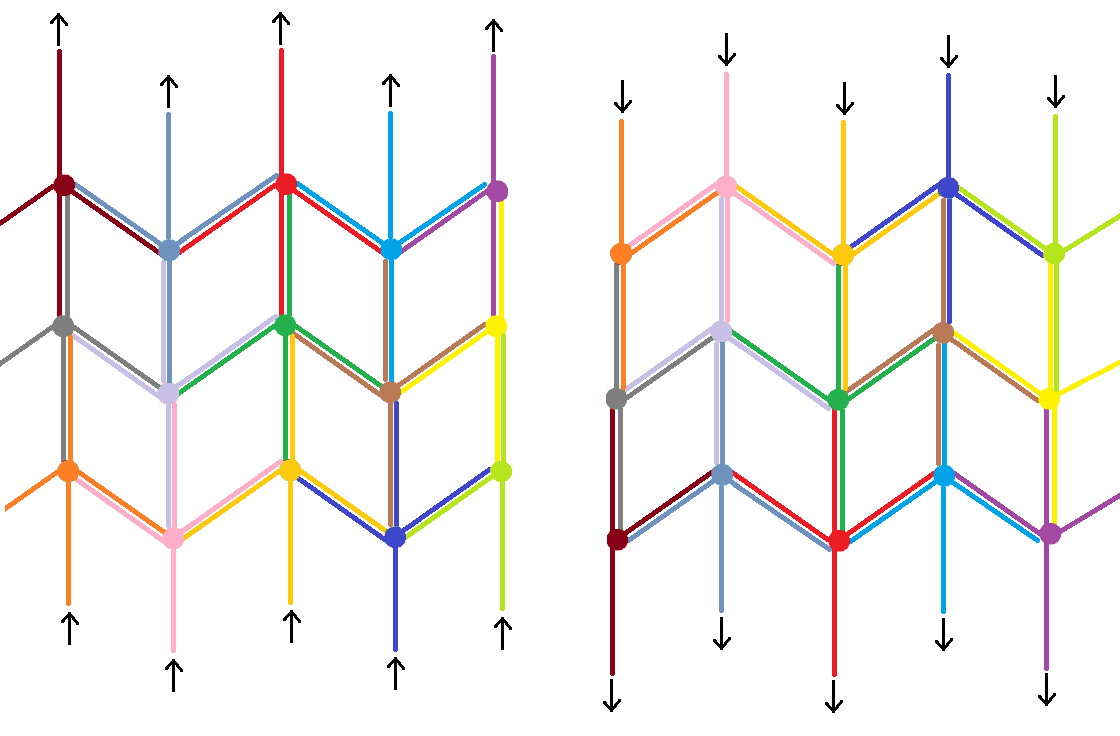
\includegraphics[scale=0.5]{./parts/img_jm/network}
\caption[Scheme of the topology]{Scheme of the topology of the network, where each dot is a satellite, each line a data link and the arrows indicate the direction that each orbital plane moves}
\label{Scheme of the topology}
\end{figure}

\paragraph{}The idea behind this configuration is that if a satellite node fails, the data has two more nodes to travel to. Since the position of the nodes in the same orbital plane do not vary relatively to a satellite in the same plane, the two links do not need to be very powerful, since the antenna range can be very narrow. The problem lies with tha two satellites in the adjacent planes, which position will vary relative to the satellite node. This will require two antennas with a range of 120º aproximately.